\chapter{Technology}\label{cha:tech}
%\begin{preprompt}
%Indicates your competence with the tools (often software packages such as TensorFlow, PyTorch, etc.) that will be the foundation of your thesis code. At this point in time, you should FULLY understand those tools, be able to CLEARLY explain them, and be able to run some prototypes related to your final project goals. For example, if you plan to use TensorFlow to implement a complex Boltzmann Machine on a complex problem, you should be able to hack up a prototype of a SIMPLE Boltzmann Machine on a SIMPLE task at this point.
%\end{preprompt}

The software implementation for this project is written in Python using the PyTorch library~\parencite{NEURIPS2019_9015} for all computational tasks.
PyTorch includes sub packages for handling the entire deep learning pipeline, i.e.~all sections shown in Figure~\ref{fig:sys}.
PyTorch is a relatively new framework, but has quickly become on of the most popular tools, especially in research.
The two main reasons for this is the \textit{pythonic} API design and its \textit{dynamic computational graph}.
The API is designed from the bottom up to integrate into the already established python data science ecosystem as well as to follow the common design goals of being clear and consistent.
One of the most complicated aspects of training neural networks is computing the derivatives for all the parameters.
All modern frameworks perform automatic differentiation using a \textit{computational graph} which tracks the computations applied to the tensors through the forward pass.
The gradients are then calculated by following this graph from the Loss and back through to the input.
Most frameworks operate using a \textit{static} graph which is calculated and stored before the training can start.
PyTorch instead uses a \textit{dynamic} approach where the computational graph is calculated at runtime with each forward pass, allowing the model to potentially change structure.
This property is not something this implementation drawn any obvious benefits, but it results in a very modular design patters, making it relatively straight forward to implement any model using the library as intended.  

\section{Model}\label{sec:model}
As stated in Section~\ref{cha:method}, a prototype of the model has been implemented.
This implementation is based on the original model, with slight modifications inspired by an implementation made by NVINIA\footnote{Released under the Apache 2.0 License, available at this \href{https://github.com/NVIDIA/DeepLearningExamples/tree/master/PyTorch/Detection/SSD}{URL:} \url{https://github.com/NVIDIA/DeepLearningExamples/tree/master/PyTorch/Detection/SSD}}, the basic structure is shown in Figure~\ref{fig:model}.
For the implementation we divide the model into four parts.
First we have the feature extraction network, which feeds into an \textit{auxiliary structure} which gradually steps down the dimensions of the feature map.
Finally we have two detection structures, one for class confidences, and one for bounding box regression.

\subsection{Architecture}
The feature extractor in the original model is the VGG-16 network~\parencite{simonyan2015deep}, but as is pointed out by the authors, this choice is arbitrary and other networks can also be used.
In our implementation we use ResNet-50~\parencite{he2015deep}.
The main reason for this being its superior performance over VGG, and the ease of witch it integrates with the auxiliary structure.
With VGG, alterations are required to transform the latter layers from FC to CNN, while with ResNet we can just truncate the network at the appropriate layer to produce a feature map with the appropriate dimensions.
PyTorch offers canonical implementations of the most popular pre-trained models as part of their API\@.

\begin{figure}[htb]
  \centering
  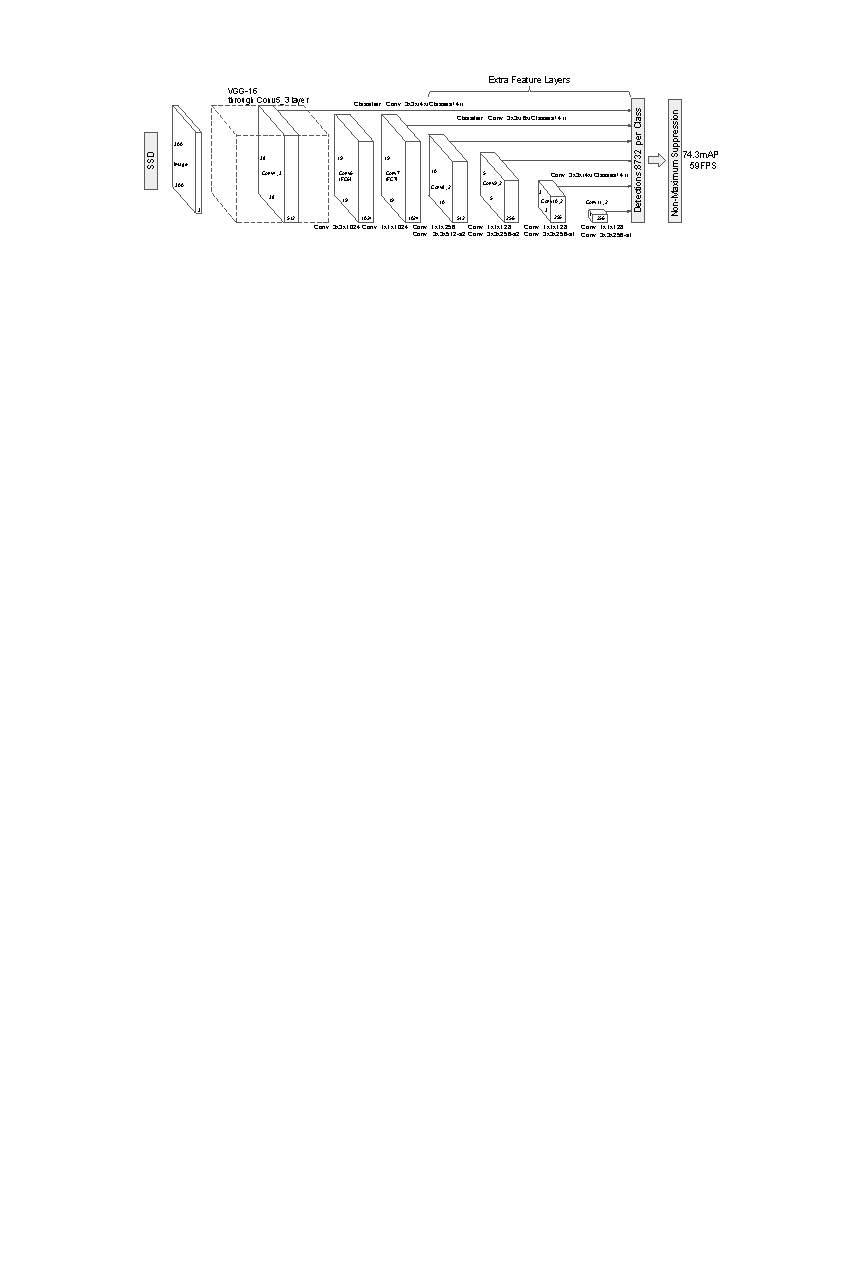
\includegraphics[width=0.9\textwidth]{figs/SSD_model.pdf}
  \caption[SSD architecture]{Visualisation of the feature layers of the SSD model as given in the original paper~\parencite{liu_ssd_2016}.
The horizontal lines denote the detection structure comprised of \(3\times 3\) convolutions for class confidences and bounding box regressions.}\label{fig:model}
\end{figure}

The auxiliary structure is implemented as a sequence of blocks where the output of each block is a feature map which is consumed by the detection structure.
Each block contains multiple convolutional layers, as specified in Figure~\ref{fig:model}.
PyTorch offers different ways to group multiple layers together so that they act as a single unit.
This makes the forward pass simple to define.

The detection structure is implemented as a sequence of distinct layers, each of which runs over one of the intermediate feature maps from the auxiliary structure.
Each localizing layer has four filters per default box, one for each of the regression parameters.
Similarly, the class prediction layers have \(C\) filters per box, one for each class with an additional layer for the background.

Because of the dynamic graph, the actual structure of the network is defined at runtime by defining a function for the forward pass.
The input is first passed through the feature extractor, it is then passed through each block of the auxiliary structure, saving each feature map.
The final output is then generated by running each feature map through the corresponding detection layer.
All the outputs from the localization and classification layers are concatenated, producing two output tensors.
The dimensions are \(\left(B,4,D\right) \) and \(\left(B,C,D\right) \) for the localization and classification outputs, respectively.
Here \(B\) is the batch size and \(D\) is the number of default boxes.


\subsection{Training objective}
Because of the default boxes, each ground truth box needs to be matched to one or more default boxes so that we have a target for the loss calculation.
SSD has a generous matching strategy where ground truths and default boxes are matched if their IoU is above 0.5.
This ensures that there are many positive examples for each ground truth.
The loss function is calculated as follows:

\[L(x,c,l,g)=\frac{1}{N}\left( L_{conf}(x,c) + \alpha L_{loc}(x,l,g)\right) \]

where \( x=\{1,0\} \) is a binary mask denoting a match between a default box and ground truth, \( N \) is the number of positive examples, \( c \) is class confidences, \( l \) is predicted boxes, and \( g \) is regressed ground truth boxes.  \( L_{loc} \) is the summed Smooth L1 loss over all positive matched bounding boxes, while \( L_{conf} \) is the SoftMax loss over multiple classes confidences, both are standard loss functions provided by PyTorch.
For the confidence loss, SSD uses \textit{hard negative mining} to balance out the negative and positive examples.
The confidence losses for all negatives are sorted and the top examples are chosen such that the ratio between positives and negatives is 1:3


\begin{figure}[htb]
  \centering
  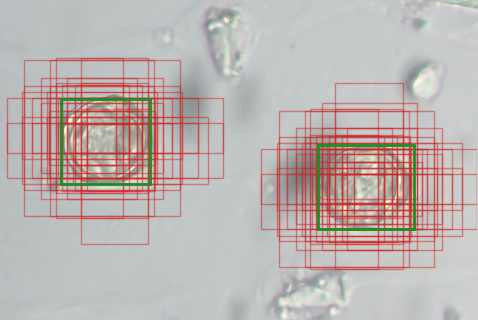
\includegraphics[width=0.5\textwidth]{figs/priors_matching}
  \caption[Default box mathching]{Visualisation of the result of the matching procedure.
In \textcolor{red}{red} are all the default boxes that are mathced to the ground truths, i.e.~those that have an IoU \( \geq 0.5 \) with a ground truth box, in \textcolor{nicegreen}{green}.}\label{fig:priors}
\end{figure}


\section{Data}
The dataset used for training the prototype is provided by~\cite{gallardo_caballero_precise_2019}.
The dataset contains a total of 390 images and 2037 ground truth boxes.
Class labels are omitted from the dataset so the model could only be trained to predict the binary prediction \textit{\{Pollen, Background\}}.
The images contain RGB with the same dimensions, \( 640\times 512 \) pixels.

\begin{figure}[htbp]
  \centering
  \begin{subfigure}[b]{0.4\textwidth}
    \centering
    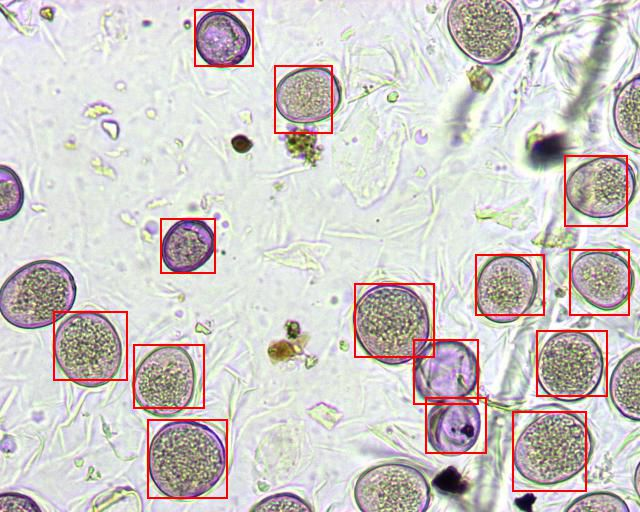
\includegraphics[width=\textwidth]{figs/ex_04}
    \vspace*{0.02\textwidth}
  \end{subfigure}%
  \hspace*{0.04\textwidth}
  \begin{subfigure}[b]{0.4\textwidth}
    \centering
    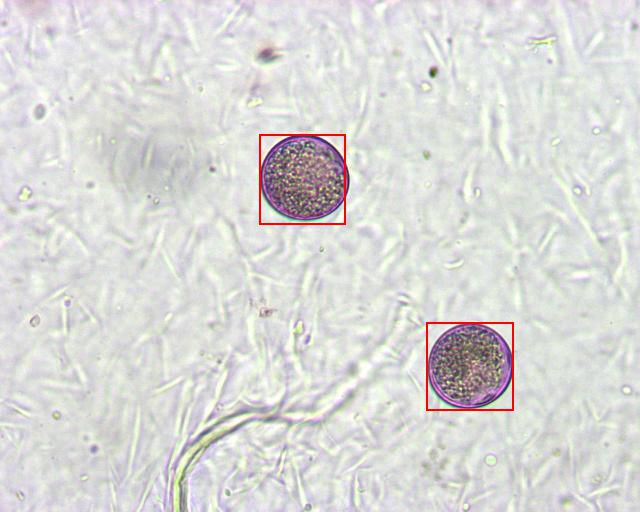
\includegraphics[width=\textwidth]{figs/ex_03}
    \vspace*{0.02\textwidth}
  \end{subfigure}

  \begin{subfigure}[t]{0.4\textwidth}
    \centering
    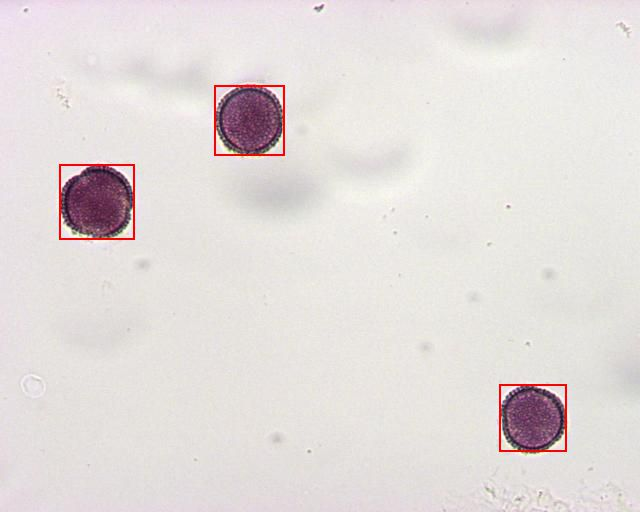
\includegraphics[width=\textwidth]{figs/ex_02}
  \end{subfigure}%
  \hspace*{0.04\textwidth}
  \begin{subfigure}[t]{0.4\textwidth}
    \centering
    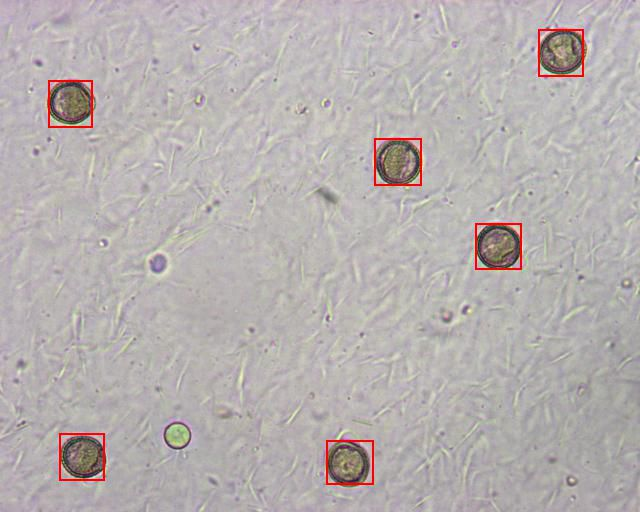
\includegraphics[width=\textwidth]{figs/ex_01}
  \end{subfigure}
  \caption[Examples from dataset]{
    Examples from the training data.
    The images vary in background and lighting conditions.
    Ground truths in \textcolor{red}{red}.}\label{fig:training}
\end{figure}


\subsection{Augmentations}
The augmentations where inspired by the original SSD implementation.
Augmentations are vitaly important with a data set this small.
The following procedure was used for the training procedure:
\begin{enumerate}
  \item Crop to 300px square containing \( \geq 1 \) ground truth box.
  \item With an independently calculated 50\% chance do any/all of the following:
  \begin{enumerate}
  \item Horizontal flip.
  \item Vertical flip.
  \item Shuffle channels.
  \item Colour shift (brightness, contrast, and saturation).
  \end{enumerate}
\end{enumerate}

With this procedure there are 16 possible combinations of augmentations that could be applied to each image, significantly increasing the apparent size of the dataset.

\section{Preliminary Results}
The results of training the prototype model show evidence of learning, but have also revealed issues that make it very hard to measure the performance.
Examples of the predictions are given in Figure~\ref{fig:pred}.
Most of the predicted boxes are concentrated around pollen grains, but because they are too small, none of them can be classified as correct.
This result is consistently found across the test set and indicates an error somewhere in the implementation.
The cause of the issue has not been found as of writing, but is most likely due to an error in either the loss calculation.

\begin{figure}[htbp]
  \centering
  \begin{subfigure}[t]{0.4\textwidth}
    \centering
    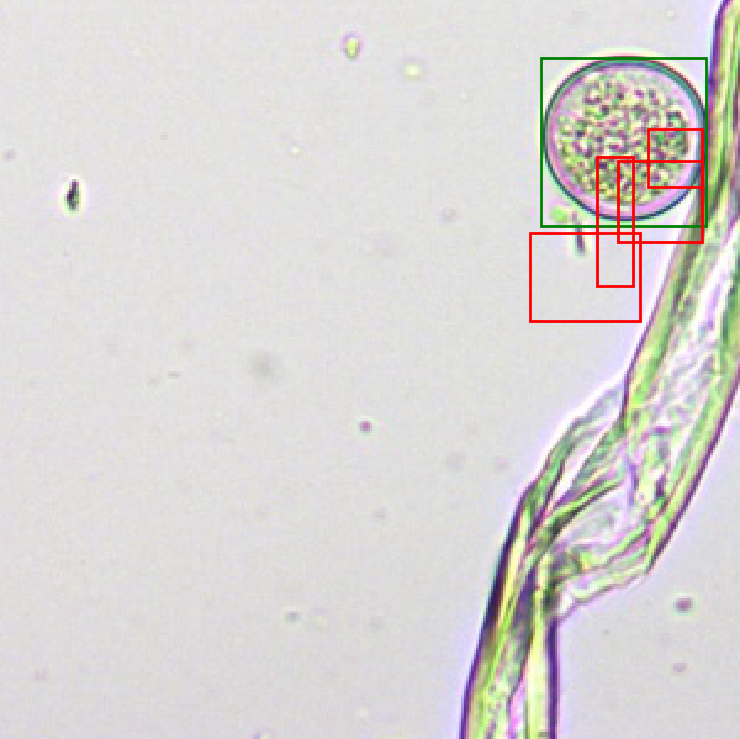
\includegraphics[width=\textwidth]{figs/infer_01}
  \end{subfigure}%
  \hspace*{0.04\textwidth}
  \begin{subfigure}[t]{0.4\textwidth}
    \centering
    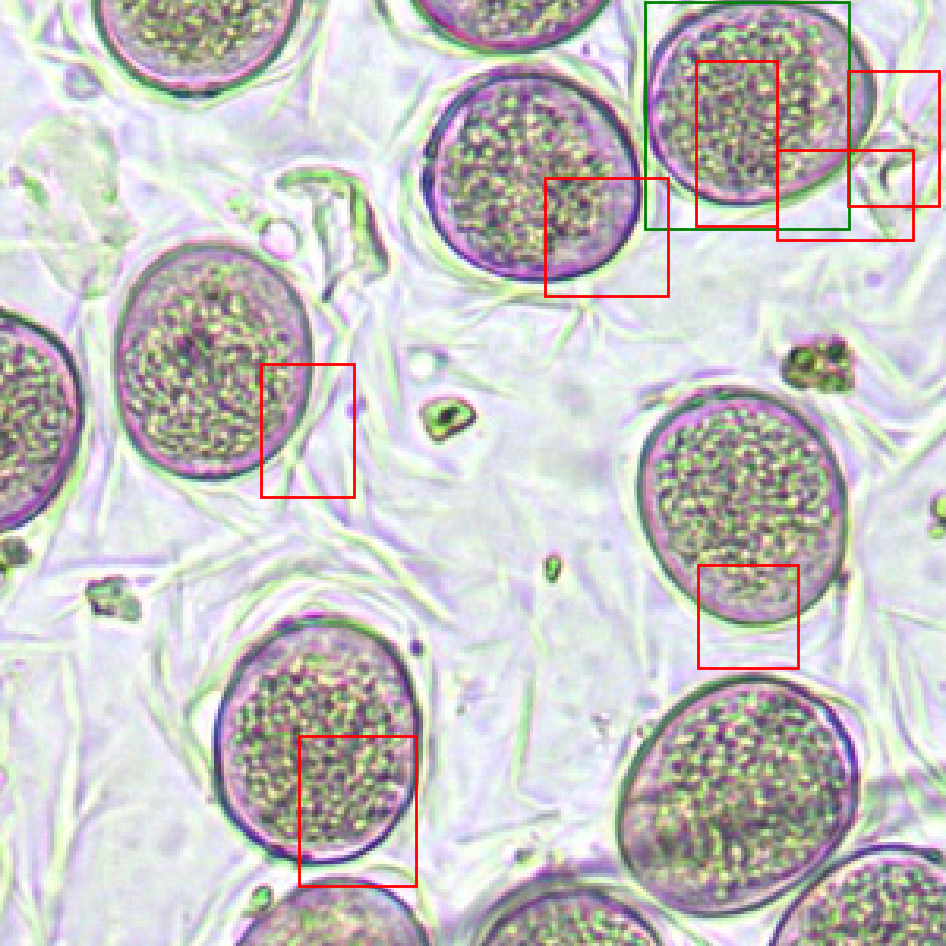
\includegraphics[width=\textwidth]{figs/infer_02}
  \end{subfigure}
  \caption[Example predictions]{Example predictions made by the trained model.
The model shows clear indications of learning, but the predictions seem to be consistently too small to be considered correct.
Predictions in \textcolor{red}{red}, ground truths in \textcolor{nicegreen}{green}.}\label{fig:pred}
\end{figure}

The preliminary results are promising, but also show that there are improvements that need to be made before any experiments can be run.
In particular, the training problems must be solved and a dataset with labelled classes must be acquired.
We will address these issues further in the next section, as we detail the plans for the remainder of this project.
